\section{Discussion}
\label{sec:discussion}


\subsection*{Tuning Searching Performance}

\scout uses ``probability threshold'' and ``misprediction tolerance'' as stopping criteria.
%We examine how they affect the search performance of \scout.\\

\subsubsection*{Probability Threshold}
\scout chooses the next configuration to evaluate
based on the probability of improvement and
stops when the probability is lower than the probability threshold $\alpha$.
\myfigure{\ref{fig:single_probability_threshold}} shows that
a higher probability threshold is pessimistic and 
terminates the search process prematurely,
hence, shorter search path
and unstable search results). 
The probability threshold presents a trade-off between
search performance and search cost.
The right threshold must consider
the reliability curve of classification methods~\cite{niculescu2005predicting}.

\subsubsection*{Misprediction Tolerance}
\scout terminates the search process if the selected configurations do not improve the current best choice (considered as a misprediction).
\scout maintains a counter of mispredictions.
A higher limit tolerates more mispredictions but yields better search performance due to more chances.
A proper limit should consider both
the size of search space and the accuracy of prediction.
In \myfigure{\ref{fig:single_misprediction_tolerance}},
we show that a higher tolerance level leads to better search performance but higher search cost.
This trade-off is similar to the probability threshold.

\begin{figure}[!htbp]
\centering
\begin{subfigure}[b]{0.4\textwidth}
    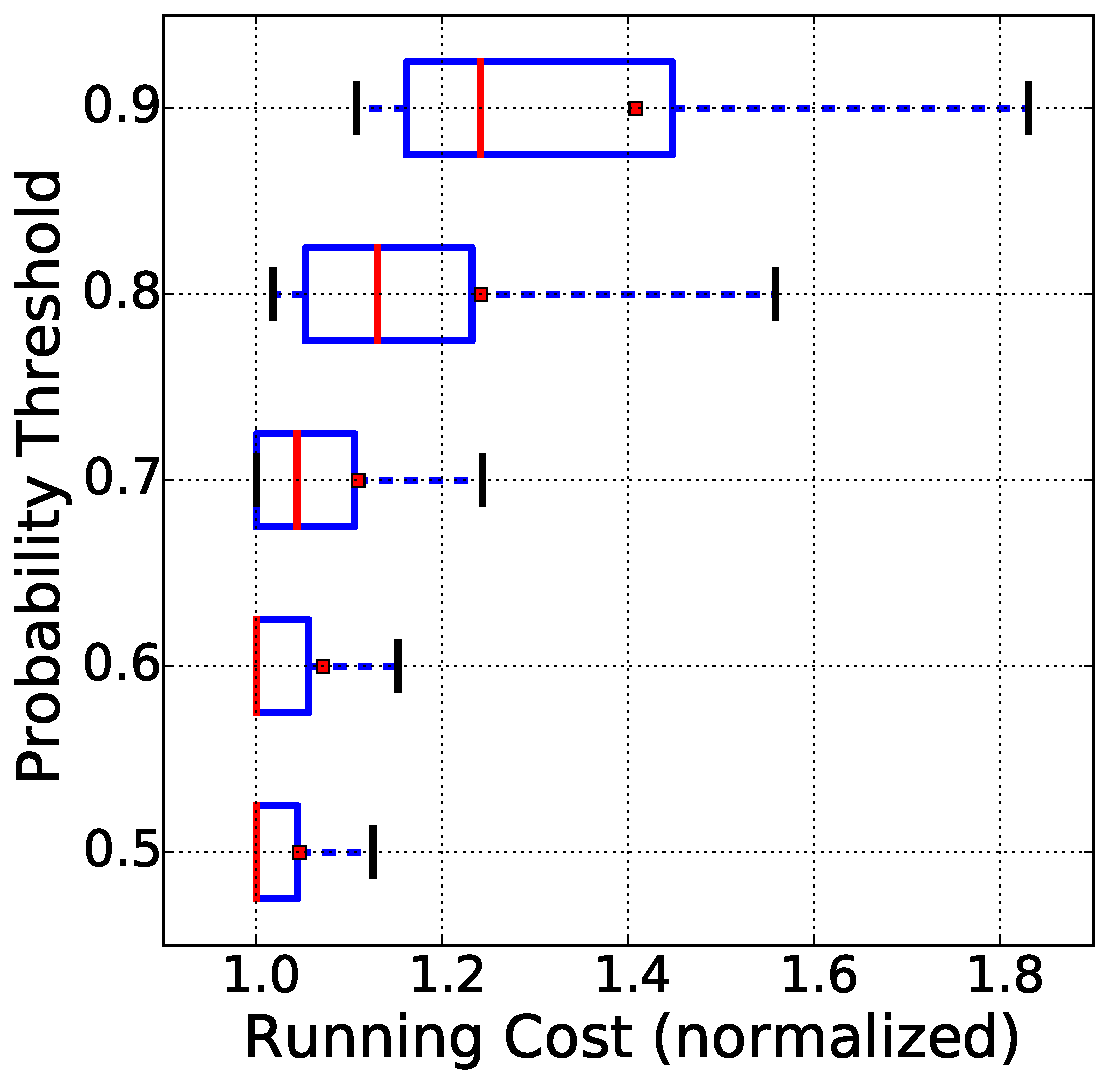
\includegraphics[width=\linewidth]{figures/single_cost_tuning_probability_performance.pdf}
    \caption{Search Performance}
    \label{fig:single_cost_tuning_threshold_performance}
\end{subfigure}
\begin{subfigure}[b]{0.4\textwidth}
    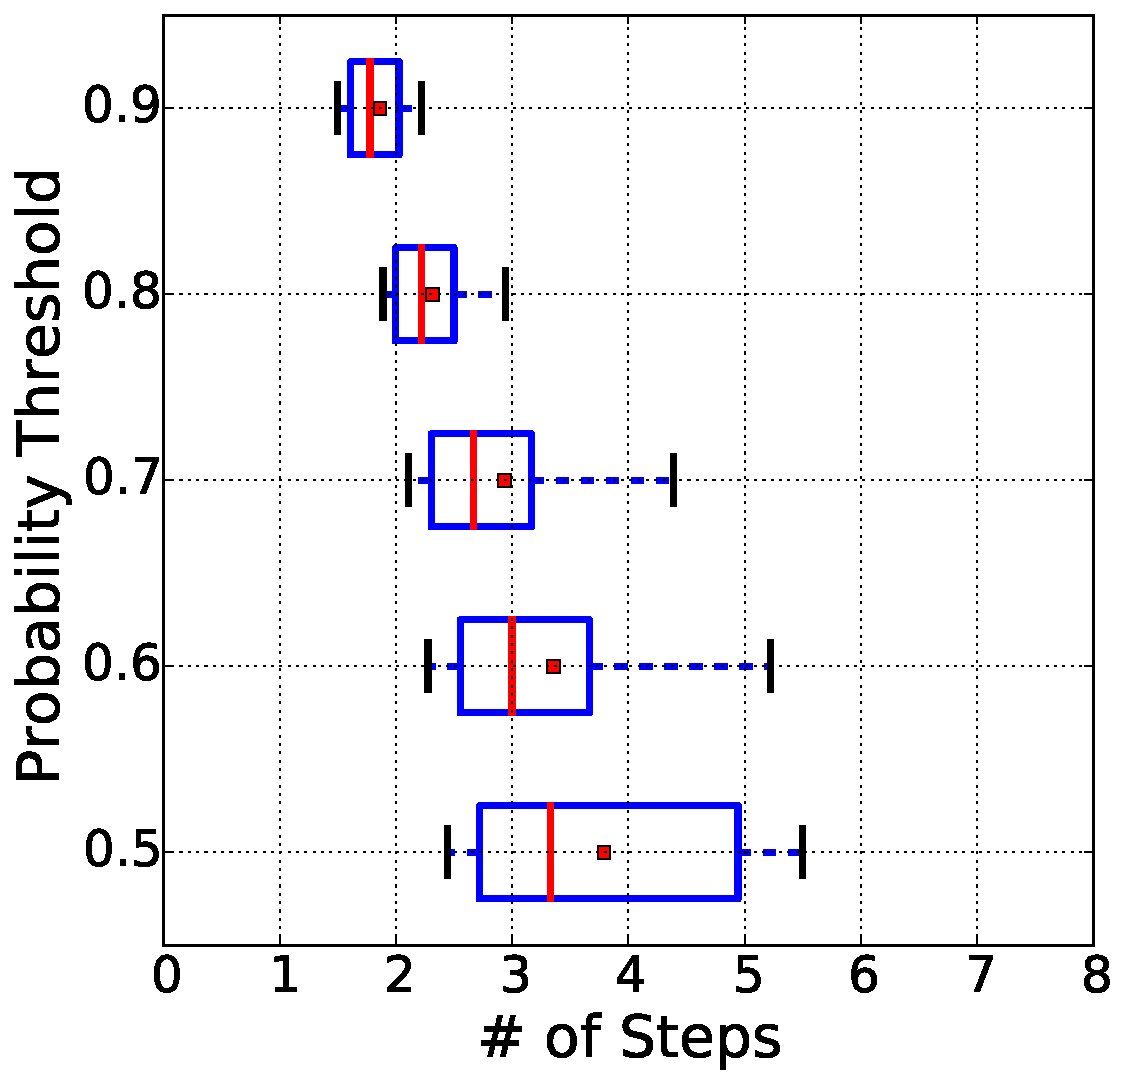
\includegraphics[width=\linewidth]{figures/single_cost_tuning_probability_steps.pdf}
    \caption{Search Cost}
    \label{fig:single_cost_tuning_threshold_steps}
\end{subfigure}
\caption{\small{\textbf{Tuning the probability threshold.} A smaller threshold generates a longer search path but ensures better search performance.}}
\label{fig:single_probability_threshold}
\end{figure}

\begin{figure}[!htbp]
\centering
\begin{subfigure}[b]{0.4\textwidth}
    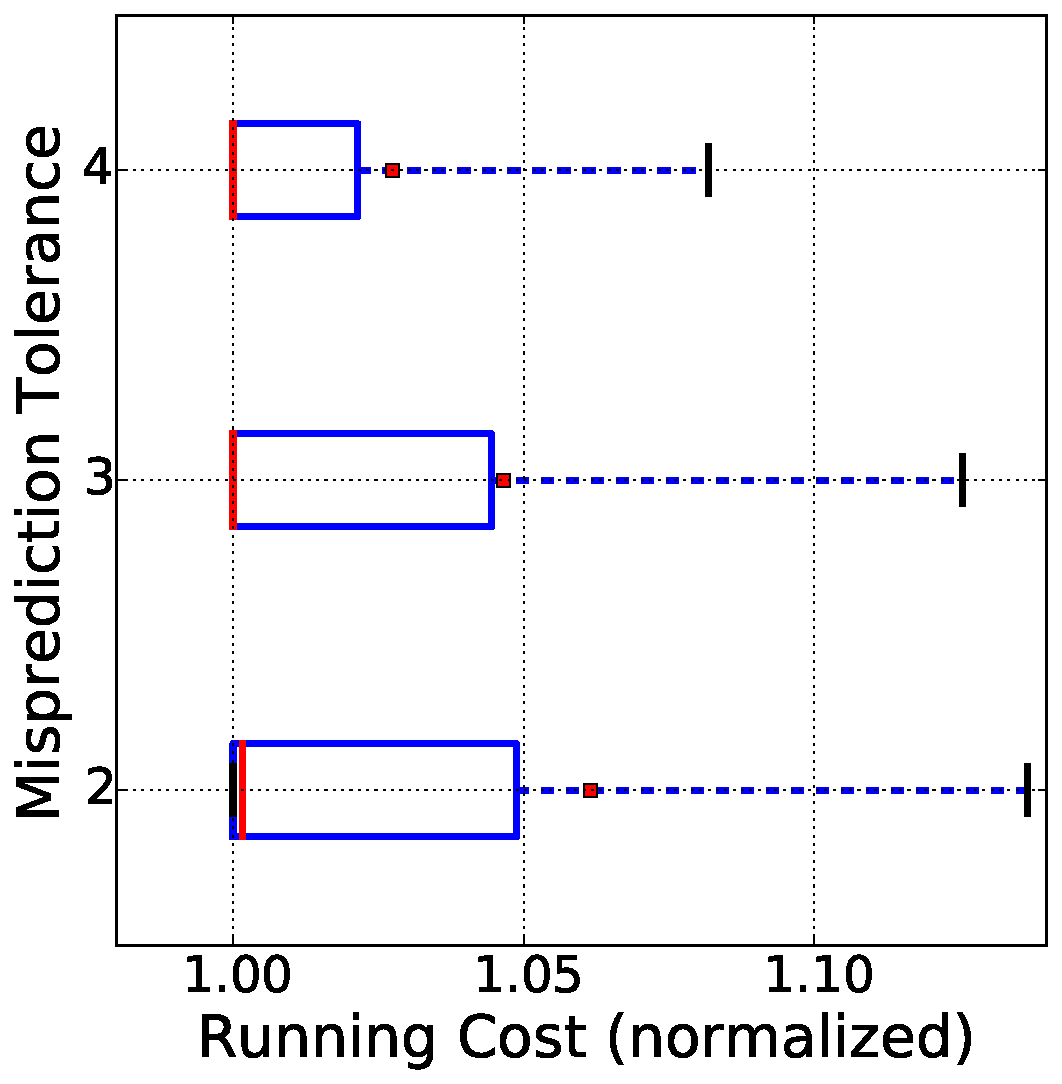
\includegraphics[width=\linewidth]{figures/single_cost_tuning_tolerance_performance.pdf}
    \caption{Search Performance}
    \label{fig:single_cost_tuning_tolerance_performance}
\end{subfigure}
\begin{subfigure}[b]{0.4\textwidth}
    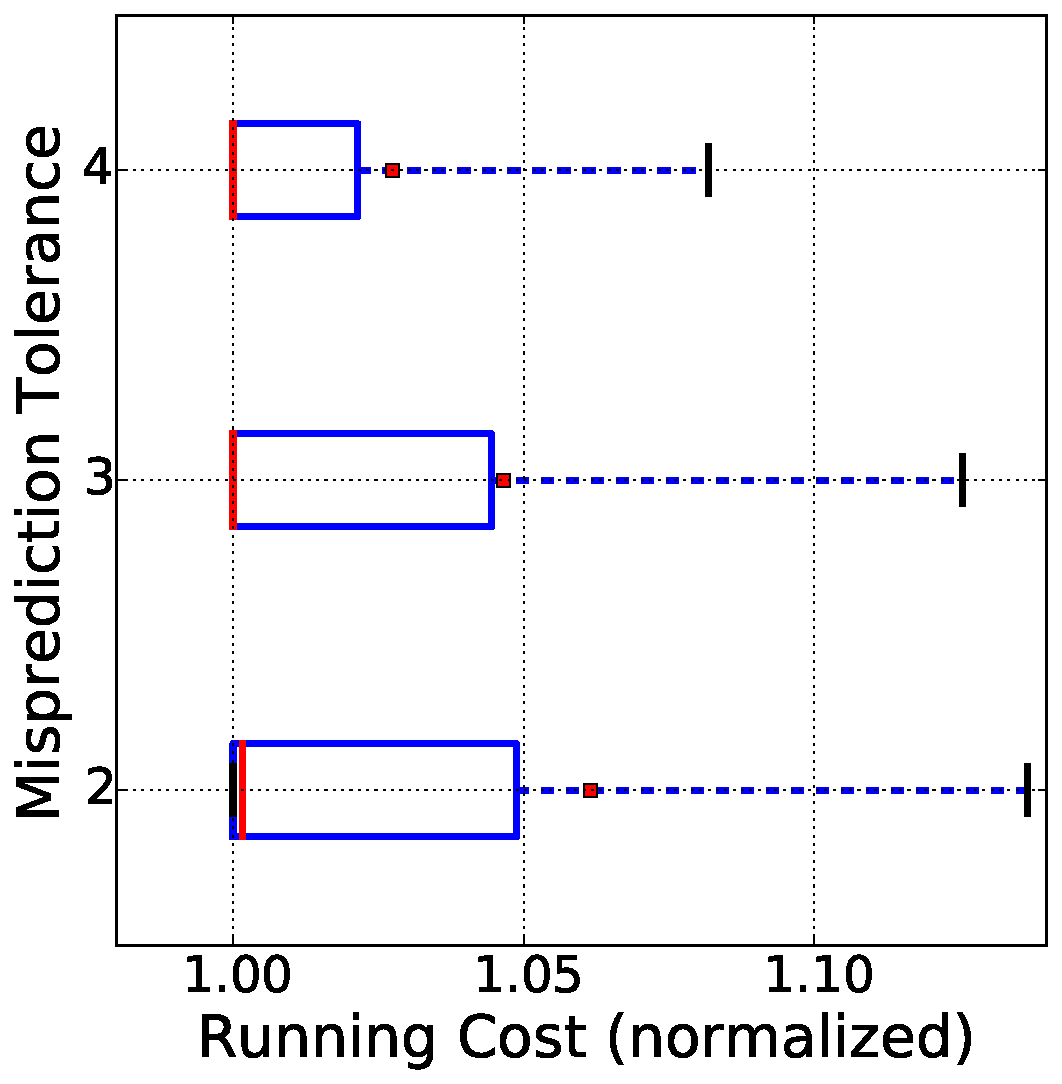
\includegraphics[width=\linewidth]{figures/single_cost_tuning_tolerance_performance.pdf}
    \caption{Search Cost}
    \label{fig:single_cost_tuning_tolerance_performance}
\end{subfigure}
\caption{\small{\textbf{Tuning the misprediction tolerance.} A higher tolerance to mispredictions generates higher search cost.}}
\label{fig:single_misprediction_tolerance}
\end{figure}


\subsection*{Alternative search strategies}
\scout generates the probability vector $P_{i}$
for each new observation (running the workload on $S_i$).
Our current search strategy only uses information from the latest observation.
\scout stores historical observations and therefore,
the next search step can be determined using several past observations.
%In \myfigure{\ref{fig:search_strategies}}, we illustrate a way to incorporate other observations.
Given two observations on $S_1$ and $S_2$ and two unevaluated configuration $S_3$ and $S_4$,
\scout generates prediction probability
$P_{13}$ and $P_{14}$ from $S_1$, and $P_{23}$ and $P_{24}$ from $S_2$.
Instead of choosing $P_{23}$ after the second step,
\scout should choose $P_{14}$ when $S_2$ is much worse than $S_1$ (due to mispredictions).
This strategy is more likely to avoid bad choices.
On the other hand, 
\scout currently relies on offline performance modeling.
Another alternative is to update the prediction model upon new observations.
For unseen workloads, this update enables \scout to improve prediction accuracy.
However, the downside is the cost of retraining the model.
An online learning method might help reduce the retraining cost.
The two possible alternatives remain as future work.

\begin{figure}[!htbp]
 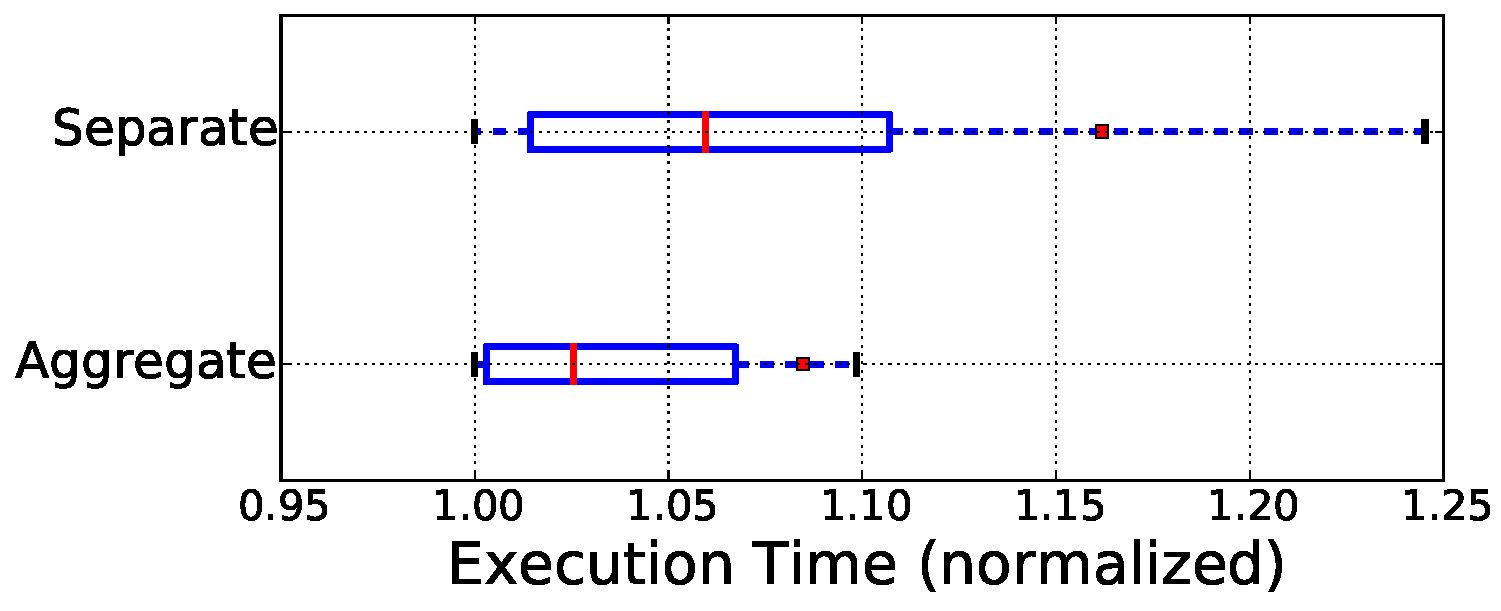
\includegraphics[width=.8\textwidth]{figures/multiple_size_of_dataset.pdf}
 \centering
 \caption{\textbf{Universal performance models.}
 Training data form multiple systems improves prediction.}
 \label{fig:prediction_accuracy_comparison}
\end{figure}

\textbf{Universal Prediction Models.}
% The performance models are built to find the best cloud configuration for a certain workload. These performance models generalize the information learned from the evaluated configurations. This helps the model to be accurate while predicting new cloud configurations. 
In prior work, the performance model needs to be retrained
for every optimization process, which leads to wasted effort.
There is a need for a modeling strategy, which becomes more accurate with experience. 
% This experienced model is useful in our setting, since measuring a new cloud configuration can be resource intensive. 
Transfer learning can be beneficial in our setting,
where the performance model can predict a new workload
using knowledge learned from optimization results of other workloads~\cite{pan2010survey}.
\scout tries to learn from other performance data so that all the experience from the past optimization process is not lost.
Figure~\ref{fig:prediction_accuracy_comparison} shows
how the performance model learned from more data (from different workloads) can
generalize better than the performance model training for a single application.
In the figure, the horizontal axis represents the execution time of the workload,
and the vertical axis shows two versions of \scout. \emph{Separate}
refers to the \scout which is trained with performance data from just
Hadoop workloads, whereas \emph{Aggregate} refers to \scout trained on Hadoop
as well as Spark workloads. We can see that \emph{Aggregate} can find cloud
configurations with better performance (lower execution time). 
\textit{Overall, the prediction model used in \scout is universal and can learn from any workload.}

\subsection*{Time-cost trade-off}
Often a
user is willing to wait longer for a result if there is a big
reduction in cost.
For example, many might be willing to trade a 20\% increase execution time for a 50\% decrease in running cost.
This is similar to the energy-time trade-off in high-performance computing~\cite{Freeh2007}.
\scout can support this scenario.
In our design, we define prediction classes based on the normalized performance of a single performance measure, \ie{time or cost}.
Previous work supports this trade-off in a similar manner~\cite{Hsu2018Arrow}.
%We instead define the classes based on the normalized performance of the product of time and cost.
%In our previous work, we show that how to support time-cost trade-off in a search-based method~\cite{Hsu2018Arrow}.
%We plan to support this feature in \scout.

